\section{Context View}

\begin{figure}[ht]
    \centering
    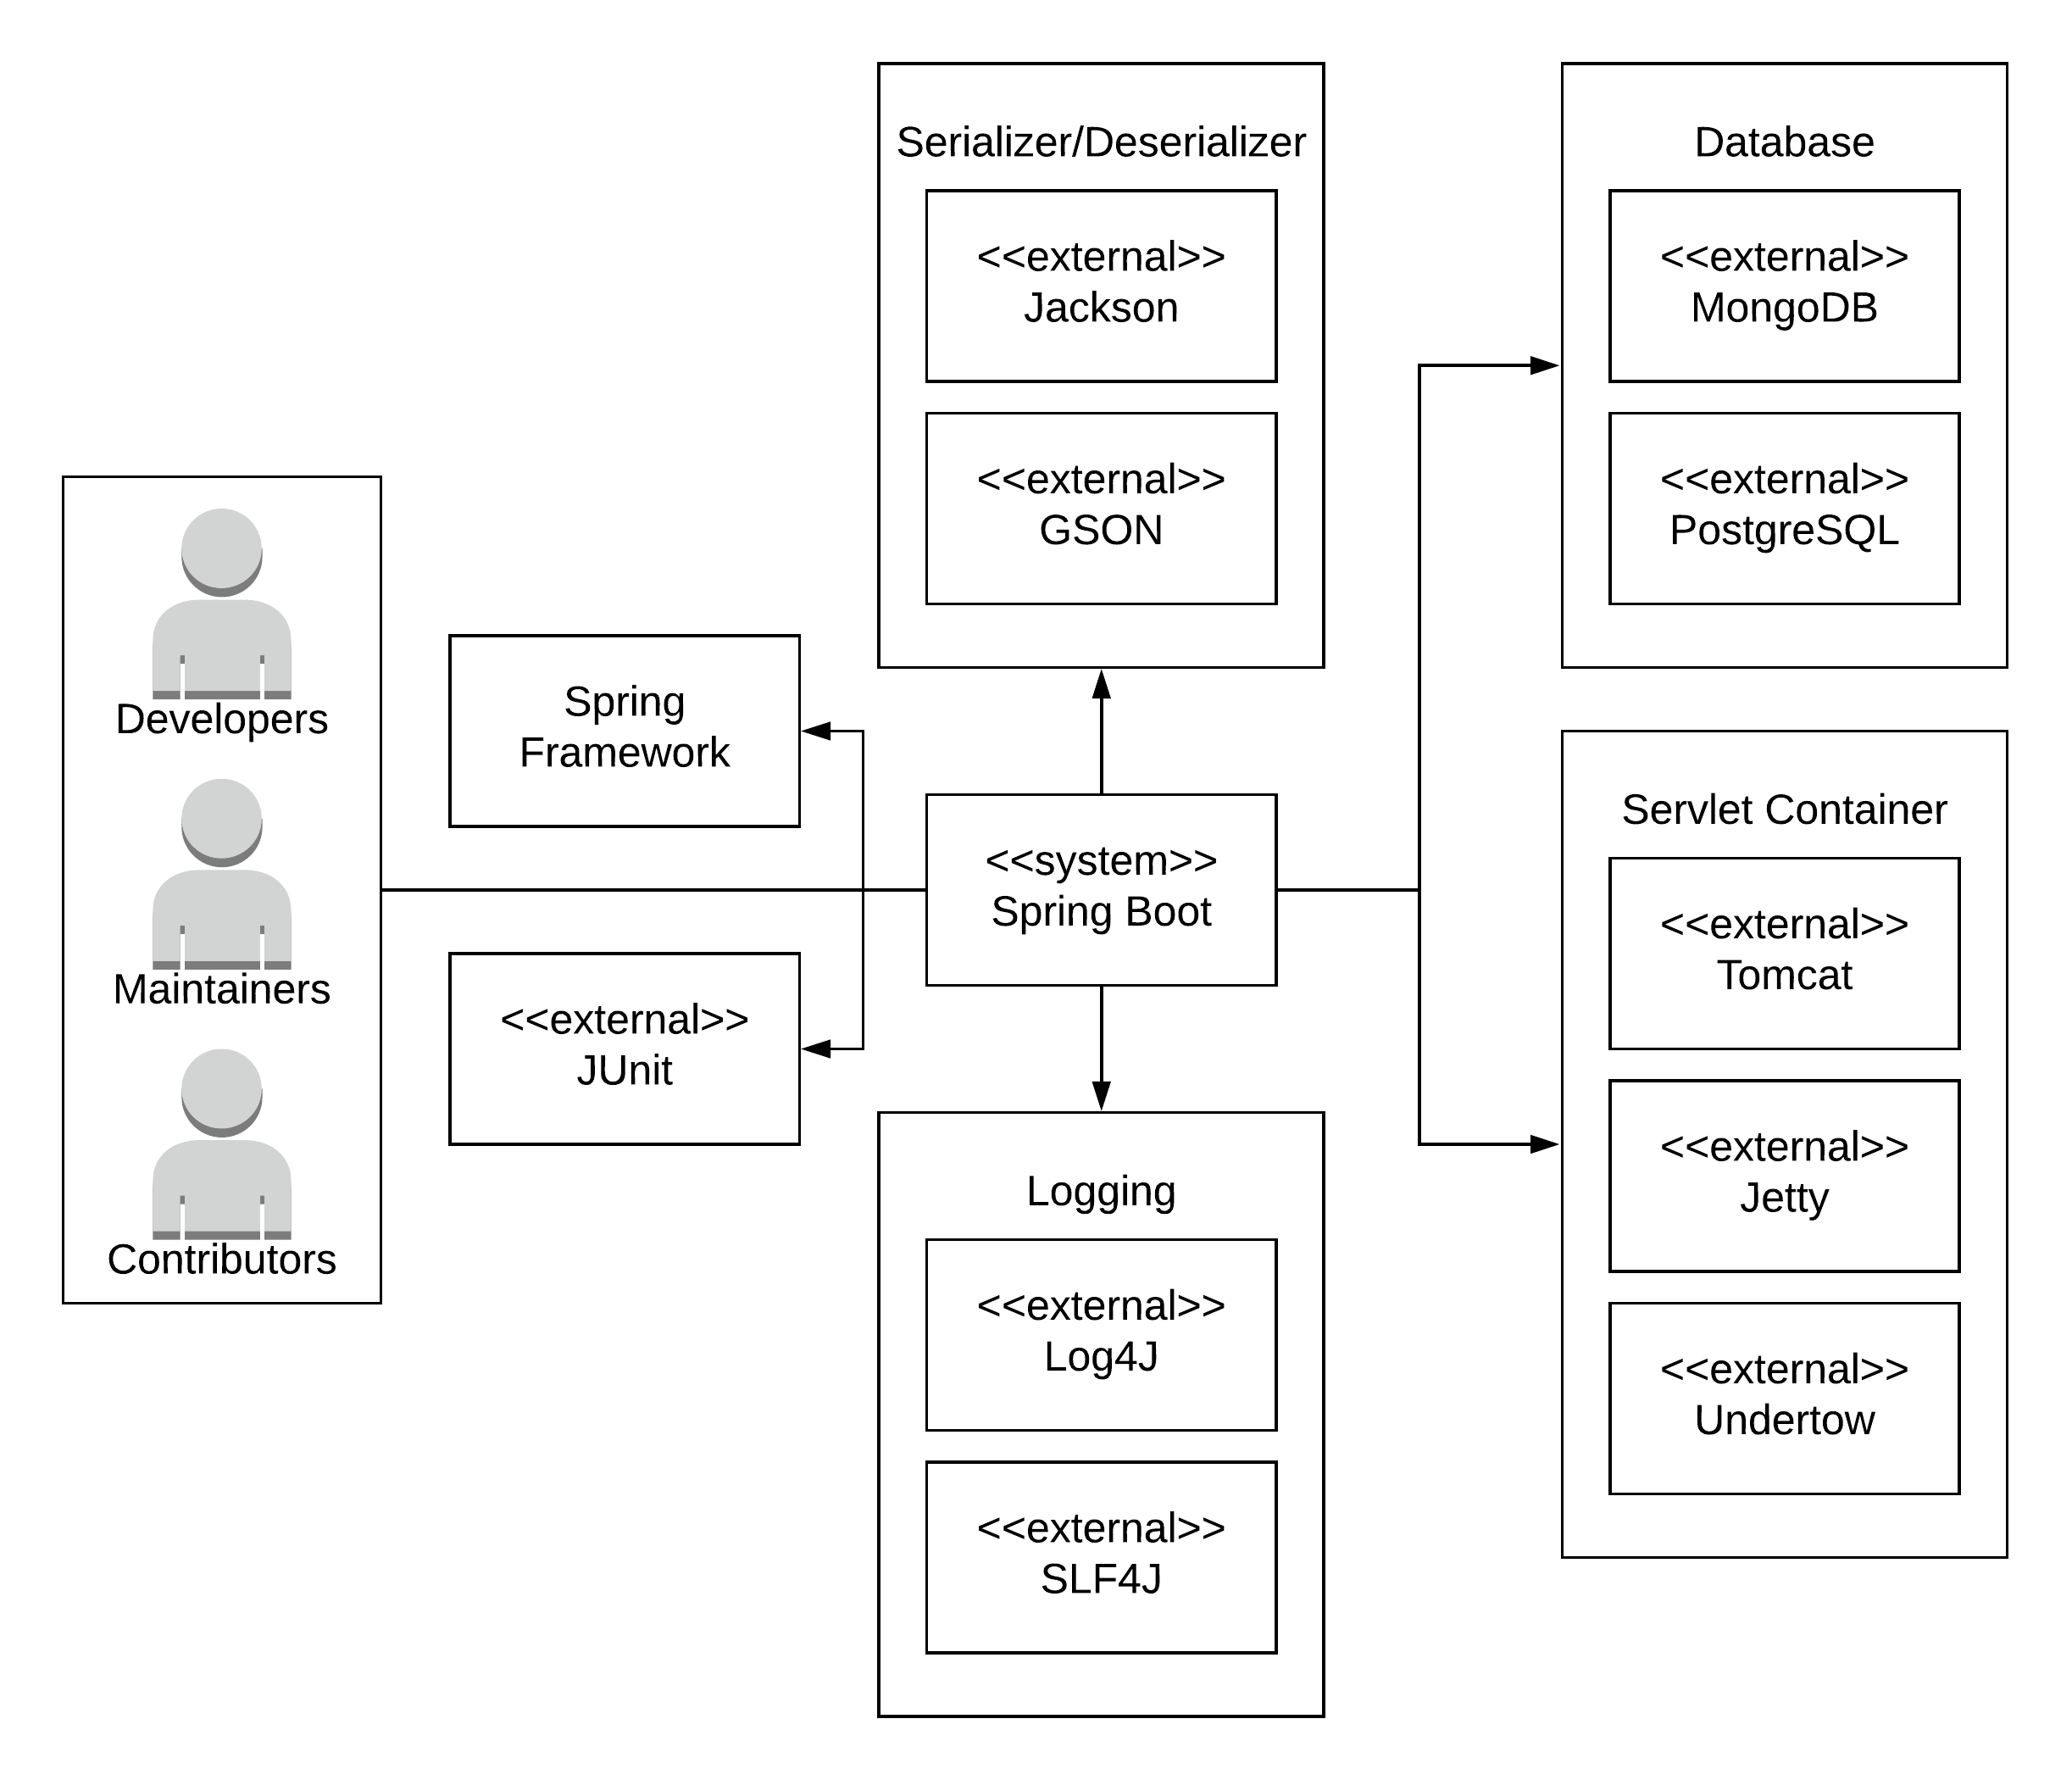
\includegraphics[width=0.75\textwidth]{content/architectural-views-top-level/context-diagram-spring-boot.png}
    \caption{Spring Boot Context Diagram}
    \label{3-context-diagram}
\end{figure}

Spring Boot has the following actors, which are listed below:

\begin{enumerate}
  \item \textbf{Developers}: Users who develop web service applications using Spring Boot.
  \item \textbf{Maintainers}: The team that overlooks the open-source Spring Boot project and develops features as well as addressing bugs and vulnerabilities.
  \item \textbf{Contributors}: The Spring community at wide that participates in improving, developing, and reporting bugs and vulnerabilities.
\end{enumerate}

Spring Boot has the following dependencies, which are listed below:

\begin{enumerate}
  \item \textbf{Spring Framework}: A Java-specific platform for developing a wide-range of applications.
  \item \textbf{JUnit}: A Java-specific testing framework for unit and integration testing
  \item \textbf{Logging}: Spring Boot has logging integration for libraries such as Log4J and SLF4J, which can provide various logging levels dependent on user informational needs (i.e. \texttt{OFF, FATAL, ERROR, WARN, INFO, DEBUG, TRACE}).
  \item \textbf{Servlet Containers}: Spring Boot by default supports three embedded servlet containers such as Tomcat, Jetty, Undertow. These containers have the ability to communicate via HTTP protocols from client to servlet.
  \item \textbf{Database}: Spring Boot has support for a variety of database systems such as MongoDB and PostgreSQL.
  \item \textbf{Serializer/Deserializer}: Spring Boot by default uses Jackson to serialize and deserialize but can use other libraries such as GSON and custom implementations

  \textit{Note: The list is not exclusive to the above list and more dependencies can be found in the official Maven repository}
\end{enumerate}

Spring Boot has six internal key components, which are listed below:

\begin{enumerate}
  \item \textbf{Actuator}: additional features to monitor and manage a Spring application in production.
  \item \textbf{Autoconfigure}: automatically configures the Spring application based on the jar dependencies.
  \item \textbf{CLI}: command-line interface for developing Spring applications.
  \item \textbf{Starters}: dependency descriptors required to enable additional Spring functionality.
  \item \textbf{Test}: annotations and utilities for testing.
  \item \textbf{Tools}: additional development support features like LiveReload.
\end{enumerate}